
%%%%%%%%%%%%%%%%%%%%%%%%%%%%%%%%%%%%%%%%%%%%%%%%%%%%%%%%%%%%%%%%%%%%%%%%%%%%%%%%
%% Capitulo
%%%%%%%%%%%%%%%%%%%%%%%%%%%%%%%%%%%%%%%%%%%%%%%%%%%%%%%%%%%%%%%%%%%%%%%%%%%%%%%%
\chapterimage{chapter_head_2.pdf} % Chapter heading image

\chapter{Historia das gafieiras}
\index{Historia das gafieiras}

%%%%%%%%%%%%%%%%%%%%%%%%%%%%%%%%%%%%%%%%%%%%%%%%%%%%%%%%%%%%%%%%%%%%%%%%%%%%%%%%
\section{Gafieira}
\label{def:Gafieira}
\index{Gafieira}
Atualmente o termo gafieira indica um baile de clube particular, com entrada paga e frequência livre. 

\begin{itemize}
\item \textbf{1979 em adiante:} Se entende que as gafieiras são locais de lazer 
e dança onde existe bom comportamento e muita compostura,
em perfeita integração racial; de modo que, 
a gafieira é sinônimo de baile em salão espaçoso como boa música orquestral \cite[pp. 10-11]{respeitojournalbrasil1}.

\item \textbf{1932 ate antes de 1979:} O termo gafieira foi associado a lugares de baixa ralé, onde 
se aconteciam frequentemente delitos e trágicos acontecimentos \cite[pp. 11]{gafieirajournalbrasil1} \cite[pp. 12]{gafieirajournaloradical1} \cite[pp. 10-11]{respeitojournalbrasil1}.

\item \textbf{1932:} popularização do termo gafieira, apos o
incidente entre o jornalista Romeu Arêde (Picareta) e o empresario e fiscal de salão Júlio Simões,
que provocou que  Picareta publica-se uma matéria apontando 
ao clube de Júlio como uma gafieira \cite[pp. 3 - cad. 3]{juliosimoes} 
\cite[pp. 21]{efege1974maxixe} \cite[pp. 78]{coutinho2006cronistas};
pelo que este último decidiu apelidar seu exitoso ``Elite clube'' como gafieira;
espalhando-se rapidamente esta denominação a outros clubes similares. 
Assim, o termo queda vinculado a clubes de dança da classe média,
onde eram aceitos todas as pessoas sem nenhum tipo de preconceito racial, 
prévio pago da entrada \cite[pp. 6 - cad. B]{entrevistajuliojournalbrasil1}.


\item \textbf{1917 ate 1932:} 
Inícios do uso do termo gafieira, indicando bailes populares \cite[pp. 29]{instituto1987revista} de entrada paga
ou bailes criados por motivo do carnaval; sendo que, as referencias bibliográficas
achadas são nas semanas próximas ao carnaval \cite[pp. 4]{oldgafieira1} 
\cite[pp. 7]{oldgafieira2} \cite[pp. 4]{oldgafieira3} \cite[pp. 5]{oldgafieira4},
o que mostra a notoriedade que adquiriam esses eventos, ou locais, nessas datas.
\end{itemize}

%%%%%%%%%%%%%%%%%%%%%%%%%%%%%%%%%%%%%%%%%%%%%%%%%%%%%%%%%%%%%%%%%%%%%%%%%%%%%%%%
\section{Cronologia das gafieiras}


%%%%%%%%%%%%%%%%%%%%%%%%%%%%%%%%%%%%
%\PRLsep{Bailes na década de 1800}

Seguindo o jornalista Agostinho Seixas,
entre os anos de 1847 e 1848, na Cidade Velha, no Rio de Janeiro,
já existiam  bailes e clubes recreativos, 
que hoje denominaríamos como \textbf{gafieiras} \cite[pp. 11]{respeitojournalbrasil1}.
Seixas achou como primeira referencia na suas pesquisas, que entre essas datas,
Dona Francisca Pacheco da Silva, fazia um requerimento 
à ``Excelentíssima Câmara'' (que foi concedido) para a autorização 
da sua sala de bailes, na Rua da Alfândega, 327 \cite[pp. 11]{respeitojournalbrasil1} \cite[pp. 71]{perna2002samba};
este requerimento foi catalogado como sala de danças, 
com a característica de ter entrada paga.
Seguindo o fiscal que acompanhava o requerimento,
ele não achava artigo que regulamentasse esse tipo de local 
de diversão ou dança; lembremos que nessa época
o padrão era ter clubes fechados que tinham um determinado número de sócios \cite[pp. 11,12]{respeitojournalbrasil1}.



%%%%%%%%%%%%%%%%%%%%%%%%%%%%%%%%%%%%
\PRLsep{Bailes na década de 1900}


Para inícios do século XX, podiam ser achadas varias associações para negros e mestiços, 
com distintas  finalidades, como: sociedades beneficentes, literárias, dramáticas, esportivas 
e as ``sociedades dançantes e recreativas'' abertas a um público geral
\cite[pp. 154-155]{neres1999negro} \cite[pp. 71]{de2008bexiga}.
Estas associações geralmente não tinham local próprio, 
e tinham que alugar espaços que terminavam sendo salões de velhos sobrados
ou similares \cite[pp. 154-155]{neres1999negro} \cite[pp. 49]{diniz2003almanaque}.
Entre as organizações sociais recreativas mais comuns da época tínhamos, 
os cordões\footnote{Os cordões eram grupos festivos de dança e música, 
com pessoas mascaradas com figurinos de reis, de
bichos, de pajens, de guarda, etc., tocando instrumentos africanos \cite[pp. 23-24]{fernandes2001escolas}},
os ranchos\footnote{Quando os cordões desapareceram estes se transformam em ranchos (depois de 1908), 
agregaram instrumentos de corda e metais, e inciou a ser tocado a marcha-rancho,
os ranchos eram cordoes mais civilizados \cite[pp. 24]{fernandes2001escolas}} 
e os zé-pereiras\footnote{ Uma sociedade recreativa do ``Ze-pereira''
é uma sociedade dedicada a dança carnavalesca \cite[pp. 10]{simoesjournalbrasil1}} 
\cite[pp. 10]{simoesjournalbrasil1}.


Uma destas sociedades de dança do inícios do seculo XX, que agora definiríamos como gafieira, 
foi a ``Sociedade de Danças Clovis Invencivel''\footnote{Em algumas versões 
``Clovis Invencivel'' é referenciado como ``Clowns Invencíveis'' \cite[pp. 3 - cad. 3]{juliosimoes} ou 
``Clovis Invencíveis'' \cite[pp. 10]{simoesjournalbrasil1}}, 
esta foi fundada no Rio de Janeiro em 1906, 
na qual eram populares concursos de valsa, polca ou quadrilha \cite[pp. 6 - cad. B]{entrevistajuliojournalbrasil1}.
O dono da ideia da criação destes concursos foi um muito jovem e fiscal do salão, Júlio Simões,
que a seus 16 anos pensou numa sociedade de dança diferente dos da época,
que se dedicavam a ``bater bumbo'' (bailes carnavalescos ou de zé-pereira), 
a uma dedicada a ``arrasta-pés'' (bailes de salão) 
\cite[pp. 6 - cad. B]{entrevistajuliojournalbrasil1} \cite[pp. 3 - cad. 3]{juliosimoes} \cite[pp. 10]{simoesjournalbrasil1}.

Com o surgir dos lugares de baile, em 1915 \cite[pp. 1 - cad. B]{gafieira2000reis},  
Júlio Simões, foi chamado pelos sócios\footnote{Os 
sócios fundadores da ``Kanaga do Japão'' são José Constantino da Silva 
e José de Paiva Brito \cite[pp. 1 - cad. B]{gafieira2000reis}} da ``Kanaga do Japão'' para dirigir seu novo clube,
lugar de grande tradição no Rio de Janeiro, e muito popular na época,
no qual o conjunto encarregado de animar o local era chefado por Sinhô e Bulhões de Carvalho,
que receberam o título popular de ``reis da valsa'',
com torneios de dança que duravam ate 55 
minutos dançando uma valsa rápida \cite[pp. 3 - cad. 3]{juliosimoes} \cite[pp. 1 - cad. B]{gafieira2000reis} \cite[pp. 6 - cad. B]{entrevistajuliojournalbrasil1}.
Nas festas comandadas por Júlio, era comum ver dançar samba, polca, 
valsa e quadrilha, que ele mesmo marcava no salão \cite[pp. 1 - cad. B]{gafieira2000reis}. 


Para o ano 1930, estas sociedades dançantes tinham ganhado muita popularidade. 
Assim, apos a morte de um socio e o fechamento da ``Kananga do Japão'' 
em 1929 \cite[pp. 3 - cad. 3]{juliosimoes}  \cite[pp. 11]{eliteinaugura} \cite[pp. 1 - cad. B]{gafieira2000reis}, 
Júlio Simões procura a Heitor Persegani e  Hilário Jovino, 
e decidem fundar o local de danças chamado ``Elite club'' \cite[pp. 11]{eliteinaugura} \cite[pp. 13]{respeitojournalbrasil1},
agora chamado ``Elite clube'' \cite[pp. 3 - cad. 3]{juliosimoes},
na Rua Frei Caneca n. 4 - Centro, Rio de Janeiro - RJ;
sendo o 17 de julho de 1930 seu baile inaugural 
\cite[pp. 11]{eliteinaugura} \cite[pp. 3 - cad. 3]{juliosimoes} \cite[pp. 10]{simoesjournalbrasil1}.

Uma descrição de uma destas sociedades dançantes, anterior a 1931, pode ser vista no livro "O cabrocha"; 
escrita  por Jota Efegê em 1931; 
sobre a ``Sociedade Recreativa Familiar Bohemios de Botafogo'' \cite[pp. 24-26]{jotaefege},
a continuação é mostrado um extracto desse texto:
\begin{citando}%%
O salão, comquanto não fosse de grandes dimensões, era
de um tamanho regular, confinando com uma pequena saleta
onde tambem se dansava; estava bem affluido. Numa
heterogeneidade foliã, via-se desde a crioulinha blasée, sem
elegancia, desalinhada, á mulatinha pernostica de faces
avermelhadas por um carmin berrante, cabello engommado e
subjugado por travessas e grampos, num á la garçonne
forçado, mas exigido pela moda. Em meio dessas "cabrochas"
e "roxinhas", viam-se algumas moças brancas de apparencia
sobria. São as meninas que não podem fazer um vestido de
seda ou calçar sapatos de setim, para se apresentarem no
Fluminense ou no Flamengo e que nestes clubes se divertem,
ficando em evidencia por serem brancas.  %~\\
(Jota Efegê)
\end{citando}

%%%%%%%%%%%%%%%%%%%%%%%%%%%%%%%%%%%%
\PRLsep{Inícios do uso do termo gafieira}

Fazendo uma pesquisa na ``Biblioteca Digital da Fundação Biblioteca Nacional''
podemos achar referencias ao termo \textbf{gafieira} desde 1917\footnote{Mesmo 
ano em que foi lançado o samba ``Pelo telefone'', sendo um exito total no carnaval desse ano.}.


A primeira referencia pode ser vista no jornal ``O Imparcial'' (RJ),
do dia 17 de janeiro de 1917, como o título ``Batalha de confetti'',
no qual se anuncia que na rua Guimarães se terá uma grandiosa batalha,
organizada pelo ``bloco dos pesados'', conformado por \cite[pp. 4]{oldgafieira1} \cite[pp. 629]{spielmann2016reflexoes}:
\begin{citando}
Lourenço dos Santos (Lord Sorvete),\\
Antonio dos Santos (Lord Massa),\\
Antonio Lima (Lord Repinica),\\
Raul Dantas (Lord Ronqueira),\\
Almeidinha (Lord Prrrrr...!),\\
Arlindo dos Santos (\textbf{Lord Gafieira}),\\
Joaquim Mello (Lord Frango d'Agua),\\
Juvenal Branco (Lord Pé Pequeno),\\
Eudoxio dos Santos (Lord Garganta) e\\
Jorge Vença (Lord Come Bola).
\end{citando}
Pelo contexto do anuncio, e pela semelhança com os outros apelidos, 
pode-se perceber que o termo \textbf{gafieira} tem um significado alegre,
cotidiano ou extravagante, mas é difícil extrair alguma outra conclusão.

A seguinte referencia aparece um ano depois, no mesmo jornal,
no dia 8 de fevereiro de 1918, como o título ``Grande batalha de confetti'',
na qual se anuncia que a batalha é organizada pelo ``bloco da rapaziada'',
do ``\textbf{Club da Gafieira}'', a qual também terá a participação 
da \textbf{orquestra do ``Gafieira''} que tocará adoráveis tangos;
e se finaliza falando que  \cite[pp. 7]{oldgafieira2} \cite[pp. 629]{spielmann2016reflexoes}:
\begin{citando}
Serão distribuídos brindes áquelles que mais se têm distinguido nos bailes do valoroso ``\textbf{Gafieira}''.
\end{citando}
Nesta referencia, já podemos observar que a palavra gafieira é relativa à celebrações do carnaval, 
e a lugares ou eventos de bailes,
nos quais, por exemplo, se dançam tangos; 
pelo que a palavra \textbf{gafieira} é usada no nome da orquestra,
e no apelido de um integrante, o valoroso \textbf{Gafieira}.

Um ano depois na ``Gazeta de Noticias'' (RJ),
no dia 3 de março de 1919, com o título ``Club dos carnavalescos do Andarahy'' e subtitulo ``1ra Critica - A Gafieira'',
se anuncia que a ``Banda de clarins'' e a ``Banda de música'',
tocarão uma espirituosa ``charge'' aos bailes de clubs de mil réis por cabeça, 
na qual era  usada a seguinte letra \cite[pp. 5]{oldgafieira3} \cite[pp. 629]{spielmann2016reflexoes}:
\begin{citando}
Cinco tostão vale a varsa!\\
Grita o fiscal do salão:\\
Tirem as dama depressa,\\
Não perquem a casião!\\ ~\\
Sapeca o piston com força,\\
Requebra mais, já se vê!\\
Que depois da contradança,\\
A dama vai p'r'o bufê.\\ ~\\
Paga a entrada e não estrilla!!\\
Que isto aqui é uma deliça!\\
Se porte bem, seu varsista!\\
Cuidadinho e'n a poliça!...
\end{citando}
Nesta última referencia já podemos ver claramente o sentido do termo gafieira,
identificando a um lugar de dança, em especifico a esses lugares com entrada paga a mil réis por cabeça.
Para ter uma ideia de se este preço é pouco ou muito, podemos compará-lo com o 
preço do jornal em que foi publicado o texto, sendo este de 100 RS \cite[pp. 1]{oldgafieira3};
ou também por essas épocas, 
quando a entrada custava 2 mil réis o preço de uma cerveja  era  de 800 réis \cite[pp. 1 - cad. B]{gafieira2000reis}.
Outro dado interessante é o uso do termo ``fiscal de salão'', 
figura de autoridade que já estava presente 
nas sociedades dançantes do seculo XX, como por exemplo na 
``Sociedade de Danças Clovis Invencivel'' em 1906, pelo que queda claro
a que lugares se refere o termo gafieira.


Podemos ver outra noticia relativa as gafieiras, no dia 19 de janeiro de 1920, 
no jornal ``A Razão'' (RJ), no qual se
publica uma reportagem com o título 
``Charivari num club suburbano - Fechado pela policia'',
se referindo ao clube ``Fenianos de Cascadura'',
que seguindo o descrito, este clube era 
ponto de reunião de gente desclassificada, 
que realizava seus bailes os sábados e domingos,
cobrando na entrada $1\$100$ por cabeça.
O seguinte texto é uma porção daquela reportagem \cite[pp. 4]{oldgafieira4} \cite[pp. 629]{spielmann2016reflexoes}:
\begin{citando}
A policia local, que é a do $20^o$ districto,
já estava farta do trabalho que o club 
constantemente lhe dava e de receber reclamações 
dos moradores visinhos.\\
Deliberou então o delegado, dr. Coelho
Gomes, fechar o club, mais conhecido por 
``\textbf{Gafieira}'', na primeira occasião que `e apresentasse.\\
Ante-hontem, sabbado, á noite, o club 
deu o acostumado ``baile'' e ás 5 horas da 
madrugada houve, ali um ``charivari'' medonho,
que poz o largo de cascadura em polvorosa. 
\end{citando}
O termo charivari se usa para indicar música discordante, 
confusão, motim, tumulto, barafunda \cite[pp. 53]{almeida1996dicionario}, etc.
Assim, podemos ver como o termo gafieira, 
estava relacionado a clubes de dança com entrada paga,
e que era frequentado por pessoas de poucos recursos econômicos. 
Também é interessante ressaltar que as referencias achadas correspondem,
a datas próximas ao carnaval, o que mostra o vinculo ou o maior interesse 
destes locais nestas datas. 

Ainda podem ser achadas outras referencias ao termo \textbf{gafieira} na década de 1920,
nelas podemos destacar apelidos usados por professores de dança,
ou referencias de musicas com letras indicando que gafieiras 
são frequentadas por crioulas e/ou criadas.


%%%%%%%%%%%%%%%%%%%%%%%%%%%%%%%%%%%%
\PRLsep{Popularização do termo gafieira}

Seguindo o jornalista e cronista, Jota Efegê, %%Júlio Simões e o historiador,
o termo ``gafieira'' foi criado pelo cronista carnavalesco, 
Romeu Arêde\footnote{Em algumas versões está  referenciado como Romeu Aredo \cite[pp. 188]{raca1999}.}, 
também conhecido como ``Picareta'' \cite[pp. 29]{instituto1987revista}\cite[pp. 3 - cad. 3]{juliosimoes} 
\cite[pp. 21]{efege1974maxixe} \cite[pp. 78]{coutinho2006cronistas}, 
colunista da seção recreativa do ``Jornal do Brasil'' desde 1930 ate 1941
e anteriormente do vespertino ``Vanguarda'' (1922-1930) \cite[pp. 58-59]{efege1982figuras} 
\cite[pp. 6 - cad. B]{entrevistajuliojournalbrasil1};
porém não é indicada, por Jota Efegê, referencia nenhuma sobre a data de criação.
Efegê indica que o termo ``gafieira'', possivelmente deriva de 
``cabroeira''\footnote{Cabroeira: Malta de indivíduos chamados cabras, 
de capangas assalariados para assassinar ou para fazer o mal \cite{diciocabroeira}.} 
ou ``gaforinha'' \cite[pp. 3 - cad. 3]{juliosimoes}.
Por outro lado, Júlio Simões, socio e administrador do ``'Elite club', 
afirma\footnote{Seguindo a ``Revista do Instituto Histórico e Geográfico do Rio de Janeiro'' (1987),
Jota Efegê afirma que foi Romeu Arêde quem atrelou o termo gafieira aos clubes de dança no incidente no ``Elite clube''.} 
que o jornalista Romeu Arêde tinha a costume de entrar, 
comer, beber, dançar e não pagar \cite[pp.13 ]{respeitojournalbrasil1},
e que quando ele impediu ao boêmio jornalista e seus acompanhantes (5 ou 6) o ingresso no ``Elite'', 
porque a entender de Júlio o jornalista estava meio ``alegre'' devido a uns tragos a mais;
 Júlio indicou: ``Aqui tem ordem'' 
\cite[pp.13 ]{respeitojournalbrasil1} \cite[pp. 6]{gafieiraaredeout2} \cite[pp. 3 - Encontro]{gafieiraaredeout1},
indicando que só podiam passar com entrada franca ele mais uma dama ou um amigo;
o cronista então reagiu indicando a seus acompanhantes a se retirarem, 
exclamando \cite[pp. 29]{instituto1987revista} \cite[pp. 6 - Tribuna Bis]{gafieiraaredeout3}: 
\begin{citando}
Vamos embora! Isto aqui é uma gafieira!
\end{citando}
Outras referencias apontam que o que falou foi \cite[pp. 6]{gafieiraaredeout2} \cite[pp. 3 - Encontro]{gafieiraaredeout1}:
\begin{citando}
O que eu vou fazer nessa gafieira?
\end{citando}
Ao dia seguinte Picareta escreveria na sua coluna no Jornal do Brasil \cite[pp. 188]{raca1999}:
\begin{citando}
Aquele é um lugar da ralé, onde se cometem gafes em fieiras
\end{citando}
Varias referencias apontam que este incidente aconteceu em 1932 \cite[pp. 3 - Encontro]{gafieiraaredeout1} \cite[pp. 188]{raca1999}, 
porém não se menciona o dia exato. 




Assim, em qualquer das explicações da formação da palavra gafieira,
seja por ``cabroeira''+``gaforinha'' ou ``gafes''+``fieira'',
esta era uma denominação pejorativa para indicar a um local (``cabroeira'' ou ``gafes'').
É importante lembrar que o termo \textbf{gafieira}, já existia desde antes do 
incidente entre Júlio Simões e Romeu Arêde no ``Elite club'', 
especificamente se tem constância do uso desde 1917 \cite[pp. 4]{oldgafieira1},
pelo que para a data da apertura do ``Elite club'' em 1930,
este termo já estava no consciente de algumas pessoas, porém não estava popularizado;
pelo que se deduz que Romeu Arêde, por conta do incidente no ``Elite club'', 
atuou como catalisador para a popularização do termo gafieira.
%mas isto não descarta a informação de Jota Efegê que indica que foi Arêde quem criou o termo,
%pois  Efegê não menciona uma data especifica.

Júlio simões apos o incidente no ``Elite club'', 
decide devolver a piada e apelidar seu local como 
``Gafieira'', conservando o nome de clube, 
mas transformando-se na pratica em ``Gafieira Elite'' \cite[pp. 79]{moura1995tia} \cite[pp. 6 - Tribuna Bis]{gafieiraaredeout3}.
Por este incidente e suas repercussões, 
muitos autores consideram a ``Elite'' como a primeira gafieira do Brasil \cite{cabral2016elisete} \cite[pp. 84]{cabral1996escolas}.
Consequentemente, e em palavras de Jota Efegê, 
se considera a Júlio Simões como o criador das gafieiras \cite[pp. 3 - cad. 3]{juliosimoes}.

Nesse ponto da historia, 
o nome ``gafieira'' cobrou muita relevância e locais de dança apelidados como gafieiras surgiram no Rio de Janeiro;
depois de tudo, já existissem lugares com estas caraterísticas desde inícios do século XX \cite[pp. 49]{diniz2003almanaque}.
Os salões foram criadas a semelhança dos bailes de salão da classe média ou alta \cite[pp. 78]{coutinho2006cronistas}; 
porém, no caso das gafieiras, estas eram abertas ao público prévio pago da entrada.
A Figura \ref{fig:gafieiracrono} mostra a cronologia do uso da palavra gafieira para os salões de dança no Rio de Janeiro.
\begin{figure}[h]
  \centering
    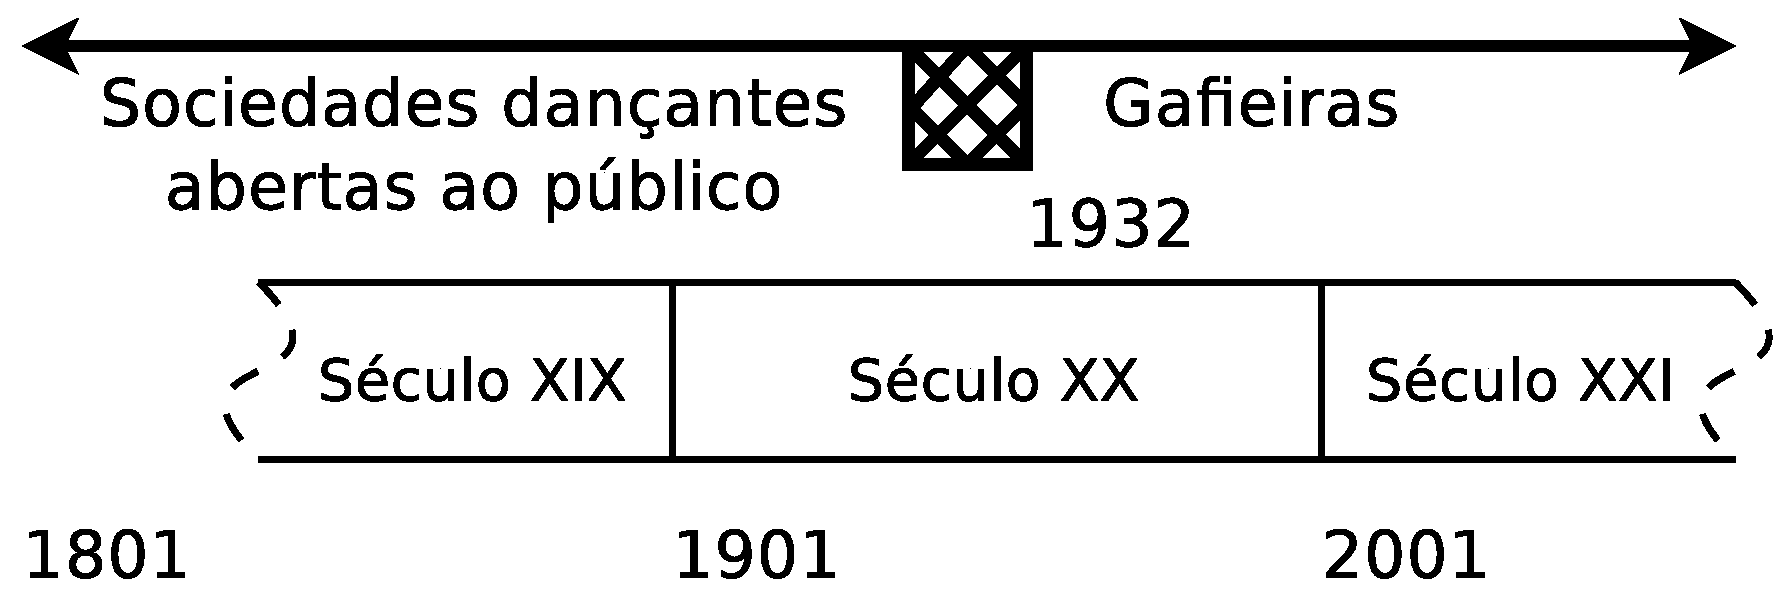
\includegraphics[width=1.0\textwidth]{chapters/cap-historia-gafieiras/gafieira-crono.eps}
  \caption{Cronologia da designação de gafieira para os salões de dança no Rio de Janeiro.}
  \label{fig:gafieiracrono}
\end{figure}

\PRLsep{Delitos vinculados com as gafieiras}

Podemos achar uma referencia ao termo gafieira no jornal ``O Radical'' (RJ),
no dia 8 de setembro de 1932 \cite[pp. 12]{gafieirajournaloradical1},
com o titular:
\begin{citando}%%
A sahida do baile: Por causa de Aracy, o estivador foi ferido á baia.\\
... Na rua Domingo Lopes, n. 243, em Madureira, está situado o club de dança Ideal, 
conhecido pelos moradores locaes por ``Gafieira''.
\end{citando} 
Ao dia seguinte, 9 de setembro de 1932, o jornal ``A Batalha'' (RJ), 
usava também a palavra ``gafieira'' para se referir ao mesmo incidente \cite[pp. 8]{gafieirajournalabatalha1}.

O ``Jornal do Brasil'', o dia 9 de janeiro de 1934, 
usa também a palavra gafieira \cite[pp. 11]{gafieirajournalbrasil1}, com o titular:
\begin{citando}%%
À porta de uma ``gafieira''.
Ainda o conflito da madrugada de domingo no largo de Madureira.
Faleceu um dos soldados no Hospital da Policia Militar. 
Ha no largo de Madureira uma sociedade dansante, mais conhecida por ``gafieira'', 
com entradas retribuidas, ondem de quando em quando, se registram conflitos, 
alguns de graves consequências...
\end{citando} 
Como é visto nas refecerias antes mostradas, e guardando semelhança com outras coincidências
posteriores que podem ser achadas na ``Biblioteca Digital da Fundação Biblioteca Nacional''; 
o termo gafieira, estava associado a lugares considerados perigosos;
isto propiciado pelo aumento do número de locais que se atribuíam este nome, junto com 
a diversidade e cultura  do seu público e administradores.
Porém, este não seria o padrão pelo qual se regiam todas as gafieiras, 
e certamente a conotação mais perigosa ou pejorativa iria mudando no tempo. 

\PRLsep{A gafieira limpa seu nome}

Por exemplo, sobre o Elite Club,  nos sabemos que funcionava as quintas, sábados e domingos,
e existia um fiscal no salão (o velho Russo)\cite[pp. 37]{gafieirajournalmanchete}, 
que fazia cumprir estritamente as normas de bom-tom, comportamento social e respeito ao ambiente, como todo clube familiar precisa ter \cite[pp. 12]{respeitojournalbrasil1}; de modo que, 
não eram admitidas damas que não estivessem de sapatos de salto alto \cite[pp. 37]{gafieirajournalmanchete};
homens embriagados não entravam e o traje indispensável era o paletó e gravata, 
ou no mínimo camisa fechada \cite[pp. 6 - cad. B]{entrevistajuliojournalbrasil1}.
O cavaleiro não podia abraçar a dama nem sentado na cadeira \cite[pp. 6 - cad. B]{entrevistajuliojournalbrasil1},
né dançar de rosto colado, ou por a mão nas costas da dama sem usar lenço \cite[pp. 10]{simoesjournalbrasil1}, 
quem fiscalizava, na porta, era um preto velho tratado por todos de ``titio''  \cite[pp. 37]{gafieirajournalmanchete}.
Se alguma regra não era cumprida, o seu Júlio, jogava a qualquer um para fora \cite[pp. 6 - cad. B]{entrevistajuliojournalbrasil1}.
Nos bailes dedicados ao padroeiro, todo 20 de janeiro, era obrigatório vestir de branco,
já seja no traje ou no vestido, incluindo sapatos e camisas \cite[pp. 37]{gafieirajournalmanchete}.
Tão grande era o censo de ordem dos frequentadores do Elite Club, 
que lhe era permitido operar estando a menos de 80 metros de um hospital,
sendo que nessa época existia a Lei n. 1.590 de 1924, 
seguindo a qual nenhuma casa de diversões podia estar a menos de 200 m de estabelecimentos hospitalares,
Ate o próprio Delegado Dulcídio Gonçalves, da Delegacia de Costumes,
dispensava-se de mandar policiar o Elite.
``À casa do Júlio não precisa de policiamento'', dizia o Delegado Dulcídio
\cite[pp. 5]{simoesjournalalutademocratica1}.


Assim, ao transcorrer dos anos, essa visão popular mais obscura da palavra gafieira foi mudando;
pelo qual o jornalista Francisco Duarte, o dia 12 de agosto de 1979,
escreve no Jornal do Brasil (RJ) sobre este assunto com o título:
``Gafieira - Tratado geral do ambiente que exige respeito'' \cite[pp. 10]{respeitojournalbrasil1}:
\begin{citando}%%
... o verbete Gafieira com o significado de baile reles, arrasta-pé, baile popular de baixa categoria.
No passado, encarada com má vontade pelos puristas do léxico e pela burguesia republicana dançante,
pode ter sido assim. Mas em 1979 -- e cabe aos dicionaristas verificar in loco --
gafieira é baile de clube particular, com entrada paga e freqüência livre, 
local de lazer e dança onde existe bom comportamento e muita compostura,
em perfeita integração racial.\\
(Francisco Duarte)
\end{citando}
Além da afirmação anterior, 
o jornalista explica como a ``Delegacia de Diversões Públicas'' classifica as casas de dança;
assim temos: 
\begin{itemize}
\item ``boates'', que são bar restaurantes com pista de dança e palco para show;
\item ``cabarés'', onde se bebe, come, dança e se tem espetáculos de variedades;
\item ``dancings'' onde se dança mediante pagamento em cartões e picotes; e 
\item ``inferninhos'' que são boates de baixa categoria, 
frequentados por pessoas de vida irregular e onde se toca música barulhenta.
\end{itemize} 
Em palavras de Duarte, ``Gafieiras são sinônimos de baile em salão espaçoso como boa música orquestral'' \cite[pp. 11]{respeitojournalbrasil1}.




%%%%%%%%%%%%%%%%%%%%%%%%%%%%%%%%%%%%%%%%%%%%%%%%%%%%%%%%%%%%%%%%%%%%%%%%%%%%%%%%
%% SUB SECTION
\section{Estatutos da gafieira}\index{Estatuto da Gafieira}
Os ``Estatutos da Gafieira'' é uma composição musical escrita, por Billy Blanco;
esta foi interpretada por primeira vez na voz de Inezita Barroso, 
numa gravação da "RCA Victor" em janeiro de 1954 \cite{musicaestatuto};
O seguinte texto mostra a letra da música numa 
versão publicada no jornal ``Cinelândia''  (RJ),
na segunda quinzena de dezembro de 1955 \cite[pp. 95]{musicaestatutojournal1955}.
\begin{citando}%%
\center{Moço! Olha o vexame!}\\
O ambiente ``ingige'' respeito!\\
Pelos estatutos da nossa gafieira\\
Dance a noite inteira, mas dance direito!\\
Aliás, pelo artigo 120,\\
O cavalheiro que fizer o seguinte:\\
Subir nas paredes, dançar de pé pro ar,\\
Morar na bebida sem querer pagar,\\
Abusar da umbigada de maneira folgazã,\\
Prejudicando hoje o bom crioulo de amanhã,\\
Será distintamente censurado!\\
Se balançar o corpo, tá na mão do delegado!\\
Balançou o corpo? tá na mão do delegado!\\
\end{citando}
O texto é uma tentativa bem-humorada do autor de descrever o que acontecia 
nas gafieiras, porém na época da escrita desta popular samba, não
existiam tais estatutos\footnote{Estatutos, no sentido de regulamento, 
ordenança o conjunto de normas legais pelas que se regula o funcionamento de uma corporação ou associação.};
existia um código de costumes sim \cite[pp. 13]{respeitojournalbrasil1} em alguns salões, 
mas cada casa de dança imponia estes no seu local a critério do fiscal do salão ou dos 
donos \cite[pp. 10]{simoesjournalbrasil1} \cite[pp. 6 - cad. B]{entrevistajuliojournalbrasil1} \cite[pp. 37]{gafieirajournalmanchete},
isto é confirmado por um depoimento realizado por 
Billy Blanco no 8 de julho de 2011 \cite[pp. 56]{depoimentobilly}; o texto a seguir
mostra um fragmento dessa entrevista.

\begin{citando}%%
"Observando os acontecimentos de uma gafieira, então, eu imaginei
coisas, porque o compositor vive muito da imaginação. E eu criava situações 
possíveis de serem acontecidas na gafieira, ou então narrava o que
acontecia realmente. Por exemplo, no [samba] Pistom de Gafieira, tinha
um cidadão que era pistonista da orquestra que sempre tocava forte para
disfarçar quando a polícia vinha chegando. Doutra feita, eu tive a ideia
de fazer o estatuto para a gafieira. Então eu humorizei, porque ninguém
dança de pé pro ar, nem sobe em parede, não é? Mas a gente cria uma
extravagância dessas para dar uma certa graça, um certo sentido à música.
Na época, não havia código nenhum, eu apenas criei aquilo e muitas gafieiras 
depois tinham esse estatuto na parede para quem quisesse cantar.
Você vê que as regras do estatuto são umas regras brincalhonas, não é?" 
~\\
(Billy Blanco)
\end{citando}

Mesmo observando que as regras propostas pelo autor tem um caráter humorístico e sarcástico,
o texto foi adotado rapidamente pelas gafieiras, como um chamado a reflexão sobre umas
normas básicas a serem tidas em conta no salão, pois tem um grau de bom senso. Por exemplo: 
A linha 7, pode ser interpretada como uma indicação a 
não fazer movimentos aéreos na pista de dança,
ou  evitar movimentos capoerísticos; tudo isto
pelo evidente espacio reduzido e compartilhado que existe na pista de dança, 
além de que os movimentos aéreos estão pensados para ser
executados em apresentações e não em danças sociais. 
A linha 8, nos lembra o respeito ao parceiro; pois a pessoa que dança precisa
estar no controle de suas faculdades físicas e mentais; 
no caso dos \hyperref[def:Condutor]{\textbf{condutores}}\footnote{\label{footlab:conducao}Nas danças sociais é comumente usado o paradigma da condução; 
no qual, no casal, uma pessoa assume o papel de \hyperref[def:Condutor]{\textbf{condutor}} dos movimentos e 
a outra pessoa assume o papel de \hyperref[def:Seguidor]{\textbf{seguidor}}, este recebe a informação da condução e retorna uma resposta corporal.}, 
para estar atentos ao salão e cuidar do seu par enquanto os movimentos são executados, 
e no caso do \hyperref[def:Seguidor]{\textbf{seguidor}}\footref{footlab:conducao} para evitar problemas
nos giros e outros movimentos que precisem  controle do eixo do corpo.
As linhas 9 e 10 indicam sobre um conjunto de expressões artísticas 
afro-brasileiras emolduradas no século XIX com o nome de ``samba umbigada'' \cite[pp. 47]{diniz2008almanaque} \cite[pp. 85]{sandroni2001feitico}; nestas danças existe
um movimento chamado ``umbigada'' \cite[pp. 50]{da2015historia} que dá nome à dança, na qual o ventre do homem e da mulher batem geralmente para indicar
a troca de dançarino; assim as linhas 9 e 10 se referem a
 evitar ``abusar'' de movimentos de umbigada que provem de danças que não eram bem vistas na época e eram consideradas gentílicas \cite[pp. 85]{sandroni2001feitico}.
Finalmente,
a linha 12 fala sobre balançar o corpo, que seguindo o contexto cultural, 
pode indicar não agir como bêbado\footnote{``Balançar o corpo; agitar, como o bebado, mal firme, e outros táes'', Diccionario da lingua portugueza, 1858 \cite[pp.296]{diccionario1858}.}, ou em outras palavras,
com pouca elegância ou respeito,
caso contrario seria levado à delegacia!.


